\section{Related Work}
Accurately predicting whether a home is occupied is a difficult task. 
People in the same home have different daily schedules; 
some go to work and others stay at home for a period of time.  
%Figure~\ref{fig_occupiedexample} illustrates an example of home occupancy. 
%The light is on. Is there any person at home? 
%When will she go out and come back? 
%\begin{figure}[h]
%\centering
%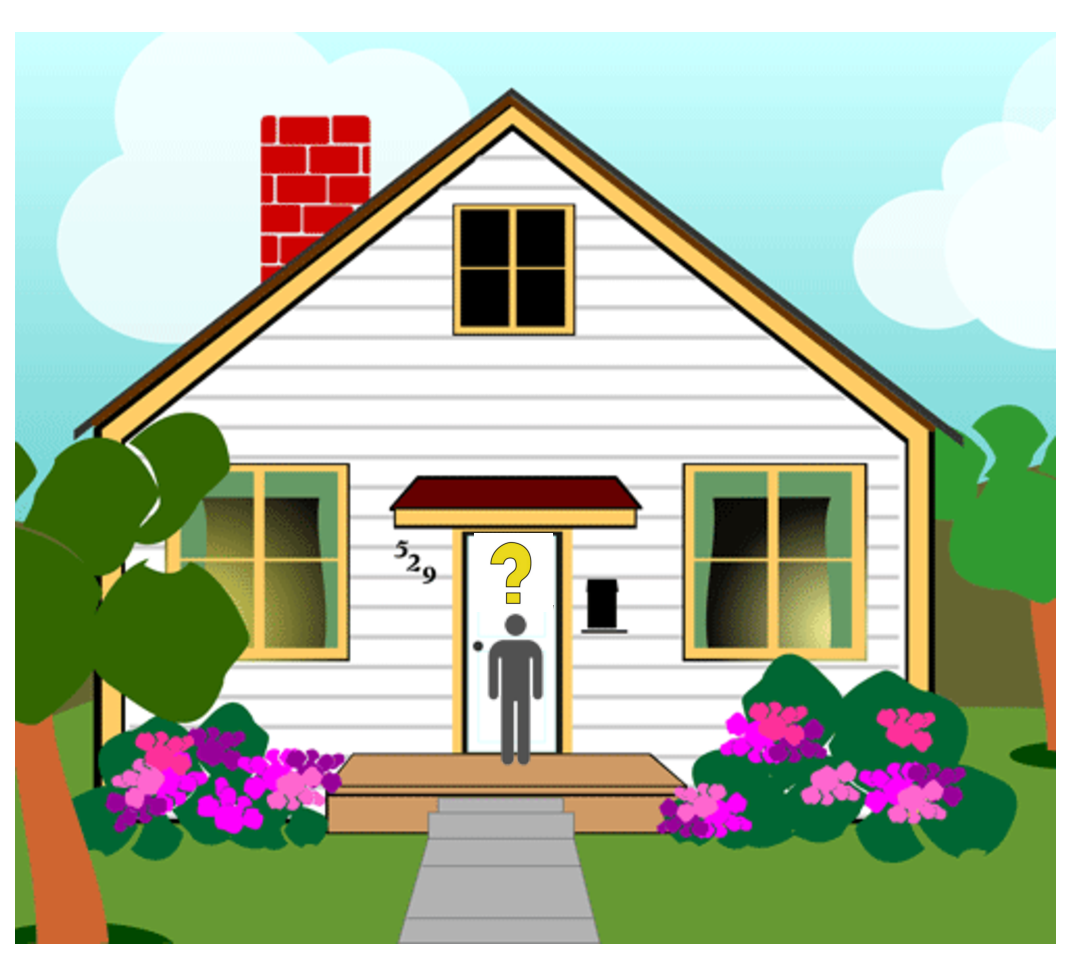
\includegraphics[width=0.35\textwidth]{adlfigs/occupied.pdf}
%\caption{Home Occupancy Example. \label{fig_occupiedexample}}
%\end{figure}
A great deal of research has been done to track the activities of people 
to infer the home occupancy. 
Researchers have made efforts to collect data by sensors, smart phones, 
the calendar, and weather information. 
Most of the approaches that model and predict occupancy primarily use sensor data to detect conditions 
such as room occupancy, use of electrical appliances, water usage, etc.
Several supervised learning approaches, such as kNN, neural networks, rule-based models, 
and Markov chain models have been used to model and predict building occupancy 
\cite{scott2011preheat,alrazgan2011learning,mahmoud2013behavioural,erickson2010occupancy,beltran2014optimal}.  
Using the kNN supervised learning algorithm and monitoring sensor data 
for a portion of the day, 
Scott et al. predict an entire day's occupancy in~\cite{scott2011preheat}. 
A neural network approach using a binary time series based on 
occupancy/unoccupancy along with exogenous input network (NARX) is 
proposed in \cite{mahmoud2013behavioural}. 
Mahmoud et al. tackle the problem by presenting a non-linear autoregressive 
model with an exogenous input (NARX) network. 
Several Markov chain models, like the blended Markov chain, 
closest distance Markov chain, 
and moving-window Markov chains are presented in \cite{erickson2010occupancy}. 
A mixture of multi-lag Markov chains was used to predict the occupancy of 
single-person offices \cite{manna2013learning}. 
In that work, the authors also compare their model with the Input Output Hidden Markov Model, 
First Order Markov Chain and the NARX neural network. 

A recent survey~\cite{kleiminger2014predicting} compares major occupancy 
predictions algorithms against the LDCC dataset~\cite{kiukkonen2010towards}, which was collected by 
GPS and other sensors. 
It shows that time-based presence probability~\cite{krumm2011learning} performs slightly better than the preheat kNN approach~\cite{scott2011preheat}. 
Since the preheat kNN approach~\cite{scott2011preheat} is more widely applicable,  
in that it can be used against both GPS and sensor datasets, 
we set it as a baseline method for comparison. 

%%%%%comment several paragraphs
\iffalse
These superseded learning approaches are classified into several categories. 
The first is on the probability density distribution of key events. 
\cite{tominaga2012unified} proposes that at a time,  a person goes out has a Bernoulli distribution. 
The second effective benchmark approach is kNN. 
kNN approach is employed in 
\cite{scott2011preheat} to predict the occupancy of the left day 
after knowing the occupancy in the partial day. 
It splits the whole day's time into 96 15-minutes intervals 
then to find the top-5 similar day in the training date. 
The average of these similarity is the predictive occupancy. 
The third is the pattern discovery by rule and neural network. 
A rule-based approach is proposed by
\cite{alrazgan2011learning}  for occupancy prediction under the frame work of Decision Guidance Query Language (DGQL). 
A variant of neural network has been proposed by 
\cite{mahmoud2010occupancy}. \cite{mahmoud2010occupancy} converts the data into binary occupancy/unoccupancy data in the first step. Then a model name non-linear autoregressive network with exogenous input (NARX) network is modeled for prediction. 
\cite{mahmoud2013behavioural} also uses binary time series with NARX network. 
The last are models related to Markov chains. 
Several Markov Chains have been compared in the paper of \cite{erickson2014occupancy}, including blended Markov Chain, closest distance Markov Chain, and the moving window Markov Chain with respect to modeling occupancy. 
\cite{erickson2010occupancy} uses moving-window markov chain for occupancy prediction. 
\cite{erickson2013poem} utilizes the markov chain model and blend markov chain model for prediction. 
\cite{beltran2014optimal} uses a blend-markov chain model for prediction. 
\cite{manna2013learning} uses mixture of multi-lag markov chains to predict the occupancy in single person offices. It compares with other previous approaches Input Output Hidden Markov Model, First order Markov Chain and NARX Neural Network. 

This paper contributes the follows:
1) formulate the problem as a temporal mining problem;
2) mine the activity patterns according to time and gap;
3) the occupancy prediction performance of this temporal mining approach works better than kNN for most cases.
\fi
